\chapter{Example}

\section{Overview}

This chapter provides a simple example of how to
\begin{itemize}
  \item include \type into a \trnsys model,
  \item export the model to an FMU and
  \item import the FMU into another application.
\end{itemize}

The example uses a simple thermal model that is exported as FMU.
The final FMU will have one input variable -- called \verb!control_signal! -- and two output variables -- called \verb!room_temperature! and \verb!mean_temperature!.
The FMU will then be used as a plant model in a simple closed-loop control system implemented in \href{https://en.wikipedia.org/wiki/Dymola}{\dymola}.
Everything needed to reproduce the steps below can be found in the subfolder \texttt{examples} of the installation directory.

\begin{figure}[h!]
\centering{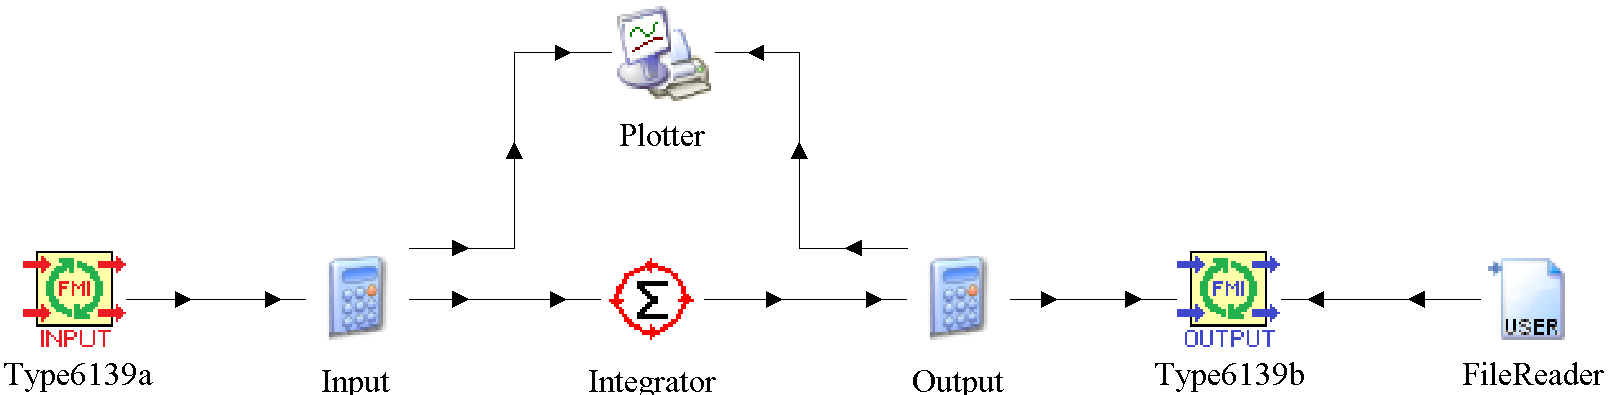
\includegraphics[width=\textwidth]{trnsys_model}}
\caption{Example \trnsys model.}
\label{fig:trnsys_model_example}
\end{figure}


\section{\trnsys model}

This example uses a very simple thermal room model that only consists of two equation blocks, an integrator block and a file reader, see Figure~\ref{fig:trnsys_model_example}.
The model is provided in file \verb!plant_room_model.tpf!, found in subfolder \verb!examples! of the installation directory.
In the following, the configuration of \typeb is explained step-by-step---the configuration for \typea is analogous.

For this example, the final FMU should have three output variables, called \texttt{room\_temperature}, \texttt{mean\_temperature} and \texttt{file\_output}.
Within the \trnsys model, these \emph{FMU output variables} shall be represented by three \emph{\typeb input variables} called \texttt{room\_temperature\_output}, \texttt{mean\_temperature\_output} and \texttt{value\_from\_file}.

To configure \typeb, proceed as follows (compare to Section~\ref{sec:export:model}):
\begin{itemize}
  \item Figure~\ref{fig:type_parameter_tab} shows the screen shot of the Proforma tab from Simulation Studio for \typeb.
  In this example, the corresponding FMU is supposed to have 2 outputs.
  Hence, the value for \texttt{number of FMI outputs} is set to~3.

  \item Consequently, the Input tab in Figure~\ref{fig:type_input_tab} shows two rows of type input variables.
  In this example they have been renamed from their default values to \texttt{room\_temperature\_output}, \texttt{mean\_temperature\_output} and \texttt{file\_output}.

  \item In the Special Cards tab, the third row specifies the FMU output variable names as a comma separated list, compare Figure~\ref{fig:type_special_cards_tab}.
  The names in this list will be matched sequentially with the input variable names specified in the Input tab.
  Hence, the numeric values associated with \typeb input variable \texttt{room\_temperature\_output} in the \trnsys model will be available via the FMU output variable \texttt{room\_temperature}, the value associated to \texttt{mean\_temperature\_output} will be available via \texttt{mean\_temperature} and the value associated to \texttt{file\_output} will be available via \texttt{value\_from\_file}.

  \item The input variables of \typeb are connected to the output variables of the \emph{Output} equation block in the usual way, see Figure~\ref{fig:type_connection}.

  \item To specify the simulation time and step size, either click the \textit{Control cards} icon in the side bar on the left or select from the menu bar on the top \textit{Assembly}~$\rightarrow$~\textit{Control cards}.
  For this example, set \textit{Simulation start time} to 0~hr, \textit{Simulation stop time} to 12~hr and \textit{Simulation time step} to 15~min.

  \item Finally, create the deck file by either clicking the \textit{Write input file} icon in the side bar on the left or select from the menu bar on the top \textit{Calculate}~$\rightarrow$~\textit{Create input file}.

\end{itemize}

\begin{figure}[h!]
\vspace*{5mm}
\centering{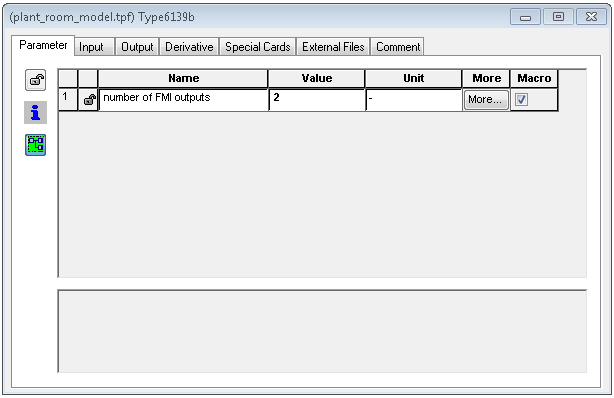
\includegraphics[width=0.95\textwidth]{type6139_parameter_tab}}
\caption{\typeb parameter tab.}
\label{fig:type_parameter_tab}
\end{figure}

\begin{figure}[h!]
\centering{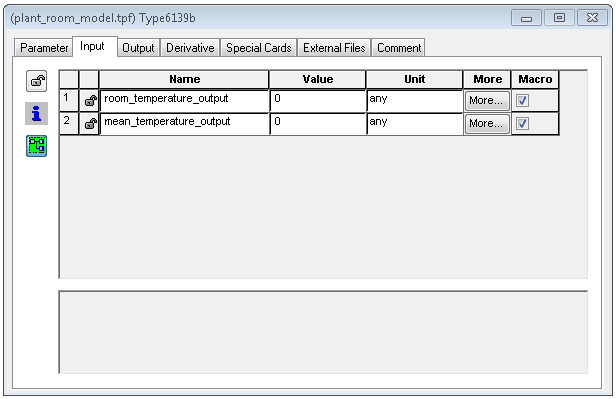
\includegraphics[width=0.95\textwidth]{type6139_input_tab}}
\caption{\typeb input tab.}
\label{fig:type_input_tab}
\end{figure}


\begin{figure}[h!]
\centering{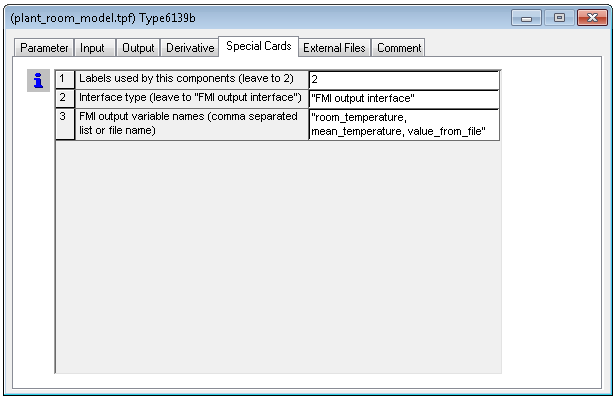
\includegraphics[width=0.95\textwidth]{type6139_special_cards_tab}}
\caption{\typeb special cards tab.}
\label{fig:type_special_cards_tab}
\end{figure}

\begin{figure}[h!]
\vspace*{5mm}\centering{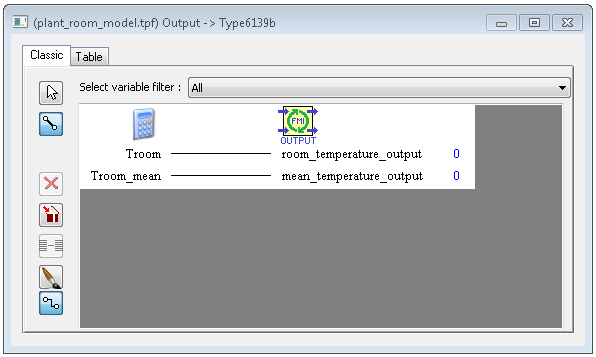
\includegraphics[width=0.95\textwidth]{type6139b_connection}}
\vspace*{5mm}\centering{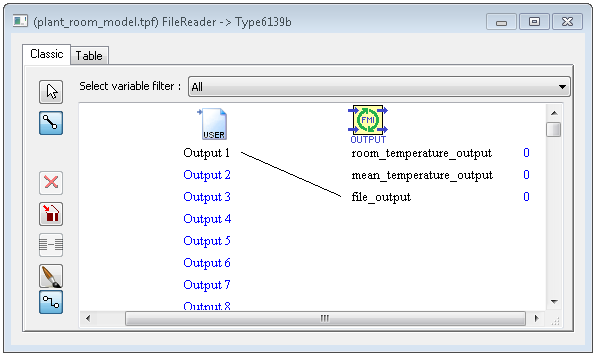
\includegraphics[width=0.95\textwidth]{type6139b_connection2}}
\caption{The inputs of \typeb are connected to the output variables of the \emph{Output} equation block and \emph{FileReader} file reader block.}
\label{fig:type_connection}
\end{figure}


\begin{figure}[h!]
\centering{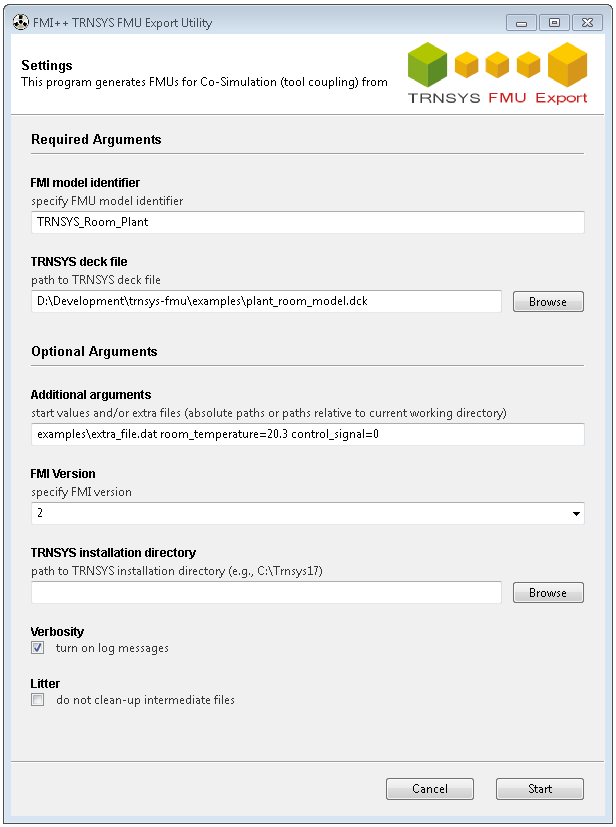
\includegraphics[width=0.95\textwidth]{trnsys_fmu_create_example_gui}}
\caption{Inputs to the graphical user interface.}
\label{fig:trnsys_fmu_create_example_gui}
\end{figure}

\begin{figure}[h!]
\centering{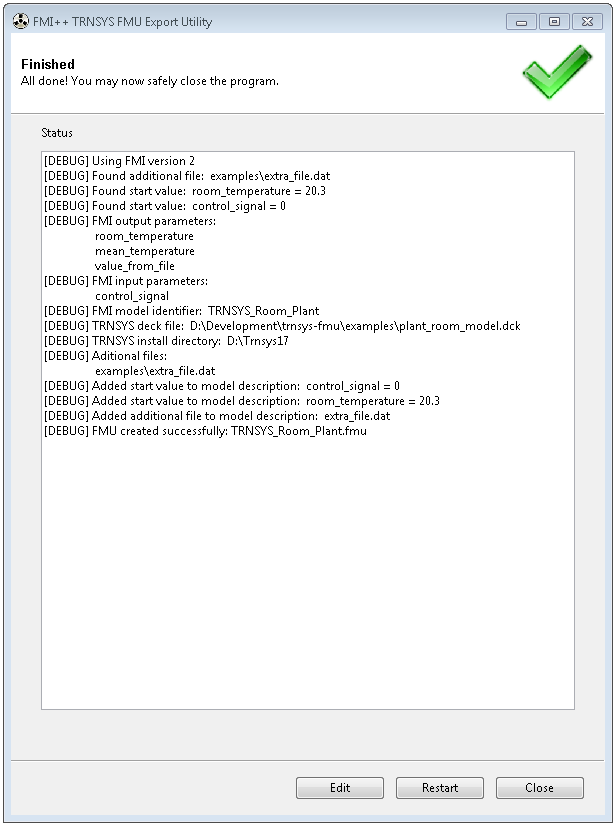
\includegraphics[width=0.95\textwidth]{trnsys_fmu_create_example_result}}
\caption{Output message from the graphical user interface.}
\label{fig:trnsys_fmu_create_example_result}
\end{figure}

\clearpage

\section{Generating the FMU}

\subsection{Graphical user interface}

Start program \texttt{trnsys\_fmu\_create.exe} in the installation directory by double-clicking it.
Then provide the following inputs (see Figure~\ref{fig:trnsys_fmu_create_example_gui}):
\begin{itemize}

  \item FMI model identifier: \textit{TRNSYS\_Room\_Plant}

  \item TRNSYS deck file: click \texttt{Browse} and select file \textit{plant\_room\_model.dck} from the examples folder

  \item Additional arguments: \textit{examples\\extra\_file.dat room\_temperature=20.3 control\_signal=0}

\end{itemize}
Then click the \texttt{Start} button to create the FMU.
This should produce the outputs shown in Figure~\ref{fig:trnsys_fmu_create_example_result}.



\subsection{Running the \python script}

Instead of using the graphical user interface, the FMU can be generated with the help of the \python script explained in Section~\ref{sec:export:command}.
For this example, the following command has to be issued in the command prompt window from the \texttt{examples} directory:
\begin{verbatim}
python.exe -v -m TRNSYS_Room_Plant -d ..\plant_room_model.dck 
          extra_file.dat room_temperature=20.3 control_signal=0
\end{verbatim}
\textbf{Attention}:
The full command is too long to be displayed in one line in this document, hence above it is split in two lines.
In the command prompt window, the command has to be written as one uninterrupted string (i.e.,~without carriage returns \keys{\return} in between).

Some comments:
\begin{itemize}
  \item The model is exported with the FMI model identifier \verb!TRNSYS_Room_Plant!, according to the value supplied to the mandatory input argument \verb!-m!.
  Hence, the FMU created will be named \verb!TRNSYS_Room_Plant.fmu!.

  \item The \python script uses the model's deck file as input.
  In this case, according to the value supplied to the mandatory input argument \verb!-d!, the deck file is stored under the name \verb!plant_room_model.dck! in subfolder \texttt{examples}.
  
  \item The start value of FMI output variable \verb!room_temperature! is specified as 20.3, compare to the results in Section~\ref{sec:example:results}.
  
  \item The optional argument \verb!-d! causes the script to output additional information. In case the scripts executes successfully, the output should look similar to the following:
\begin{verbatim}
[DEBUG] Using FMI version 2
[DEBUG] Found additional file:  examples\extra_file.dat
[DEBUG] Found start value:  room_temperature = 20.3
[DEBUG] Found start value:  control_signal = 0
[DEBUG] FMI output parameters:
         room_temperature
         mean_temperature
         value_from_file
[DEBUG] FMI input parameters:
         control_signal
[DEBUG] FMI model identifier:  TRNSYS_Room_Plant
[DEBUG] TRNSYS deck file:  examples\plant_room_model.dck
[DEBUG] TRNSYS install directory:  D:\Trnsys17
[DEBUG] Aditional files:
         examples\extra_file.dat
[DEBUG] Added start value to model description:  control_signal = 0
[DEBUG] Added start value to model description:  room_temperature = 20.3
[DEBUG] Added additional file to model description:  extra_file.dat
[DEBUG] FMU created successfully: TRNSYS_Room_Plant.fmu
\end{verbatim}

\end{itemize}


\subsection{Checking the content}

\textbf{Note}: In case of successful execution of the script, it is not necessary to check the content of the resulting FMU manually.
This section only intends to give some background information and can be skipped when working through the example.

Successfully running the script creates the FMU, i.e., a file called \verb!TRNSYS_Room_Plant.fmu!.
Since FMUs are just ZIP files, one can use standard ZIP archive processing tools (such as \href{http://www.7-zip.org/}{7-Zip}) to inspect them.
The contents of \verb!TRNSYS_Room_Plant.fmu! are as follows:
\begin{itemize}
  \item \verb!binaries!: This folder contains the shared library \verb!TRNSYS_Room_Plant.dll! in a subfolder called \verb!win32!.
  This shared library implements the coupling to \trnsys at runtime.

  \item \verb!resources!: This folder contains the deck file \verb!plant_room_model.dck! and the additional file \verb!extra_file.dat!. Both files will be loaded at runtime.

  \item \verb!modelDescription.xml!: This is an XML-based description of the model contained by the FMU.

\end{itemize}

The XML-based model description contains all relevant information about the model contained in the FMU:
\begin{itemize}
  \item the FMI model identifier and other model meta data, see XML node \texttt{fmiModelDescription}

  \item the input and output variables of the model, listed as separate \texttt{ScalarVariable} nodes

  \item information about the functionality supported by the simulation tool, see XML node \verb!CoSimulation!
  
  \item information about how to run the model with the specified simultion tool, see XML node \verb!VendorAnnotations.Tool!
\end{itemize}

For the given example, the XML model description should be very similar to the following:
\begin{verbatim}
<?xml version="1.0" encoding="UTF-8"?>
<fmiModelDescription
  xmlns:xsi="http://www.w3.org/2001/XMLSchema-instance"
  fmiVersion="2.0"
  modelName="plant_room_model"
  guid="{dde75d48-d134-11e7-9d0f-f365722dd787}"
  generationTool="FMI++ TRNSYS Export Utility"
  author="user"
  generationDateAndTime="2017-11-24T17:31:04"
  variableNamingConvention="flat"
  numberOfEventIndicators="0">
  <CoSimulation
    modelIdentifier="TRNSYS_Room_Plant"
    needsExecutionTool="false"
    canHandleVariableCommunicationStepSize="false"
    canNotUseMemoryManagementFunctions="true"
    canInterpolateInputs="false"
    maxOutputDerivativeOrder="0"
    canGetAndSetFMUstate="false"
    providesDirectionalDerivative="false"/>
  <VendorAnnotations>
    <Tool name="FMI++Export">
      <Executable
        executableURI="file:///D:/Trnsys17/exe/trnexe.exe"
        entryPointURI="fmu://resources/plant_room_model.dck"
        preArguments=""
        postArguments="/n"/>
      <File file="fmu://resources/extra_file.dat"/>
    </Tool>
  </VendorAnnotations>
  <ModelVariables>
    <ScalarVariable name="control_signal"
	  valueReference="1"
	  variability="continuous"
	  causality="input" >
      <Real start="0"/>
    </ScalarVariable>
    <ScalarVariable name="room_temperature"
	  valueReference="1001" 
	  variability="continuous" 
	  causality="output" 
	  initial="exact">
      <Real start="20.3"/>
    </ScalarVariable>
    <ScalarVariable name="mean_temperature" 
	  valueReference="1002" 
	  variability="continuous" 
	  causality="output" >
      <Real/>
    </ScalarVariable>
    <ScalarVariable name="value_from_file"
	  valueReference="1003" 
	  variability="continuous" 
	  causality="output" >
      <Real/>
    </ScalarVariable>
  </ModelVariables>
  <ModelStructure/>
</fmiModelDescription>
\end{verbatim}

\section{Using the FMU}

\subsection{\dymola model}

Subfolder \verb!examples! of the installation directory also contains a \dymola model that can be used to test the created \trnsys FMU, called \verb!trnsys_closed_loop_control_example.mo!.


This model implements a simple closed-loop control system that uses the FMU as black-box plant model, see Figure~\ref{fig:dymola_example}.
Depending on the room temperature---provided by FMU output variable \verb!room_temperature!---the controller turns the room's heating on or off---by setting the FMU input variable \verb!control_signal! to either 0~or~1.
More precisely, the model implements a hysteresis controller that turns the heater on as soon as the room temperature falls below 20.5$\,^\circ$C and turns it off when it exceeds 21.5$\,^\circ$C.

\begin{figure}[h!]
\centering{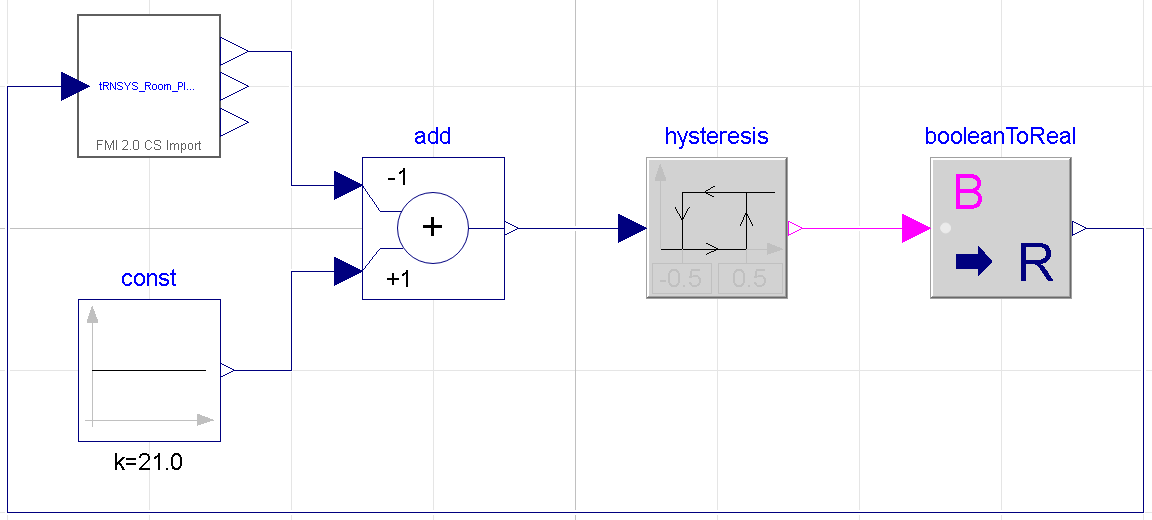
\includegraphics[width=0.99\textwidth]{dymola_example}}
\caption{\dymola example.}
\label{fig:dymola_example}
\end{figure}

To run the model, start \dymola~2018 (32-bit version), import the FMU and load the \dymola model. \textbf{Note}: Please check the \dymola documentation on how to import an FMU for Co-Simulation.


\subsection{Results}
\label{sec:example:results}

Figure~\ref{fig:dymola_output} shows the results of the simulated \dymola model.
Depicted is the room temperature as computed by \trnsys, which is kept within 21.0$\,^\circ$C~$\pm$0.5$\,^\circ$C by the \dymola controller.
Please note that the start value of the room temperature is 20.3$\,^\circ$C, as specified at the creation of the FMU.

\begin{figure}[h!]
\centering{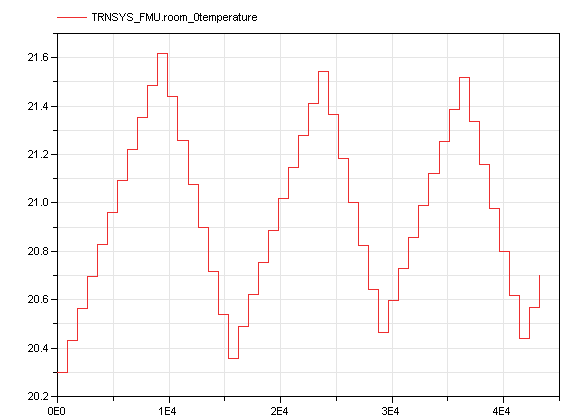
\includegraphics[width=0.99\textwidth]{dymola_output}}
\caption{Example \dymola output.}
\label{fig:dymola_output}
\end{figure}

Due to the fixed simulation step size of 15 minutes, the switching of the controller state does not happen at the exact edges of the controller's dead-band (i.e., at 20.5$\,^\circ$C and 21.5$\,^\circ$C).
Please be aware that this is not a shortcoming of the FMU itself, but due to \trnsys's restriction to fixed simulation time steps.
Such simulation artifacts are unavoidable in fixed-step co-simulation and have to be taken into account by the modeler (e.g., by choosing an adequate simulation step size).
